\chapter{2일차, 한강 하류 (서울 , 인천)}
\section{한강공원}
한강 공원은 서울특별시에서 한강종합개발계획의 일환으로 과거와 같이 깨끗한 강으로
되살리자는 목표로 만들어진 공원이다. 1982년부터 1986년까지 공사되어, 한강의 서울
지역 41.5km 구간인 하일동과 개화동을 잇는 지역이 평균 수심 2.5m, 강너비 1km 의
강으로 변했다. 강변에는 시민 휴식공원, 축구장, 배구장, 농구장, 수영장, 게이트볼장, 
체육시설, 자연학습장, 수상스키장, 수상택시승강장, 요트장, 보트장, 낚시터, 주차장 등 다양한
공간을 갖추어 시민들의 휴양지로 이용할 수 있게 되어 있다.

\begin{figure}[ht]
    \centering
    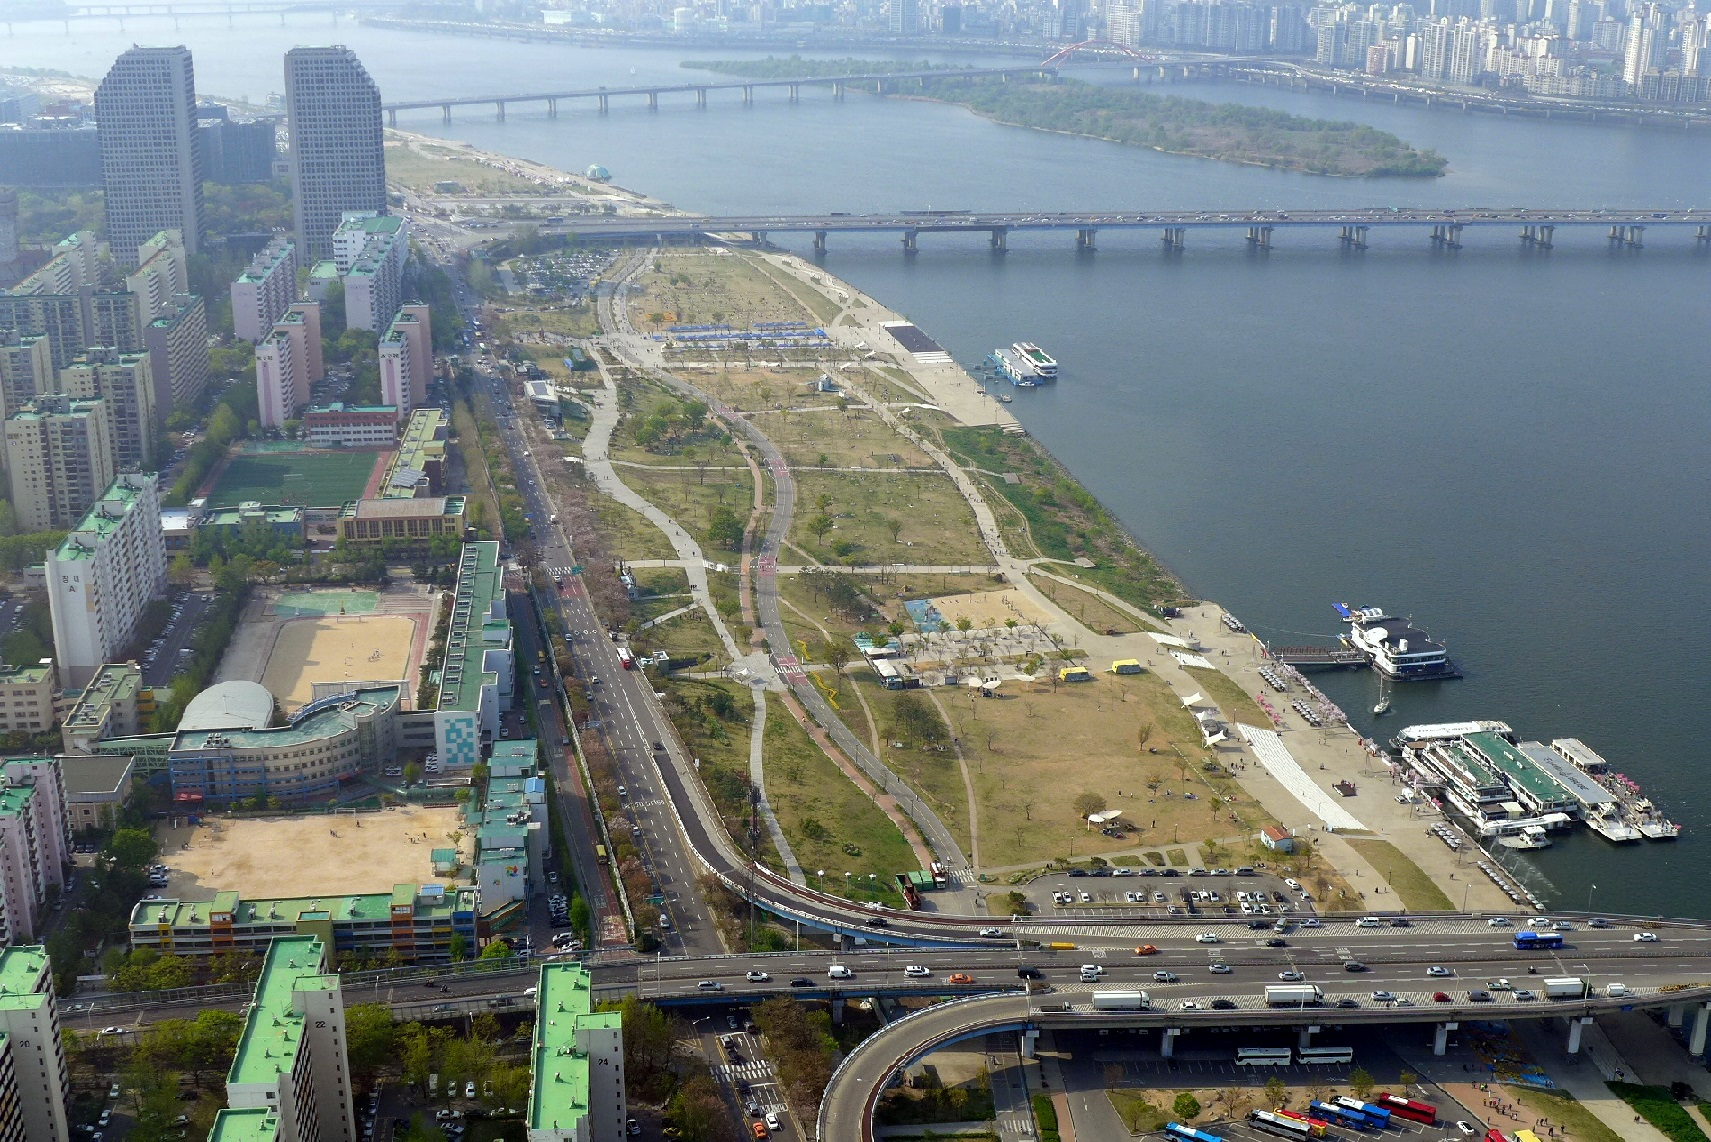
\includegraphics[width=.45\textwidth]{e_img/ww_-000_low.jpg}
    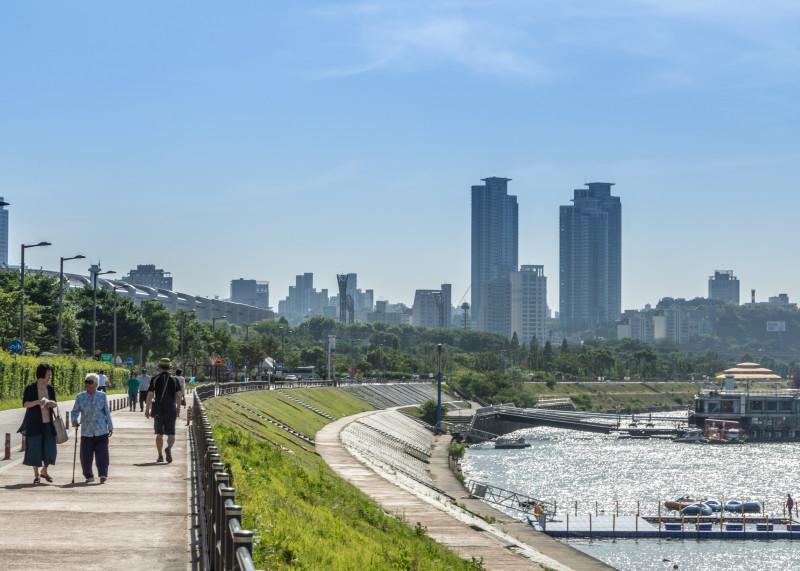
\includegraphics[width=.45\textwidth]{e_img/ww_-001.jpg}
    \caption{(좌) 드론에서 본 서울한강공원 $\quad$ (우)한강공원의 자전거길}
    \label{fig:haryu1}
\end{figure}

한강공원은 걸쳐진 지역에 따라 광나루 한강 공원, 잠실 한강 공원, 뚝섬 한강 공원,
잠원 한강 공원, 반포 한강 공원, 이촌 한강 공원, 여의도 한강 공원, 양화 한강 공원, 
망원한강 공원, 난지 한강 공원, 강서 한강 공원으로 나뉜다. 서울함 공원은 망원 한강 공원에
위치하여 있으며, 잠원 한강 공원 부근에 있는 스타벅스 서울웨이브아트센터점은 물 위에 
떠서 한강뷰를 관람할 수 있는 한강의 대표적인 명소다.

\begin{figure}[ht]
    \centering
    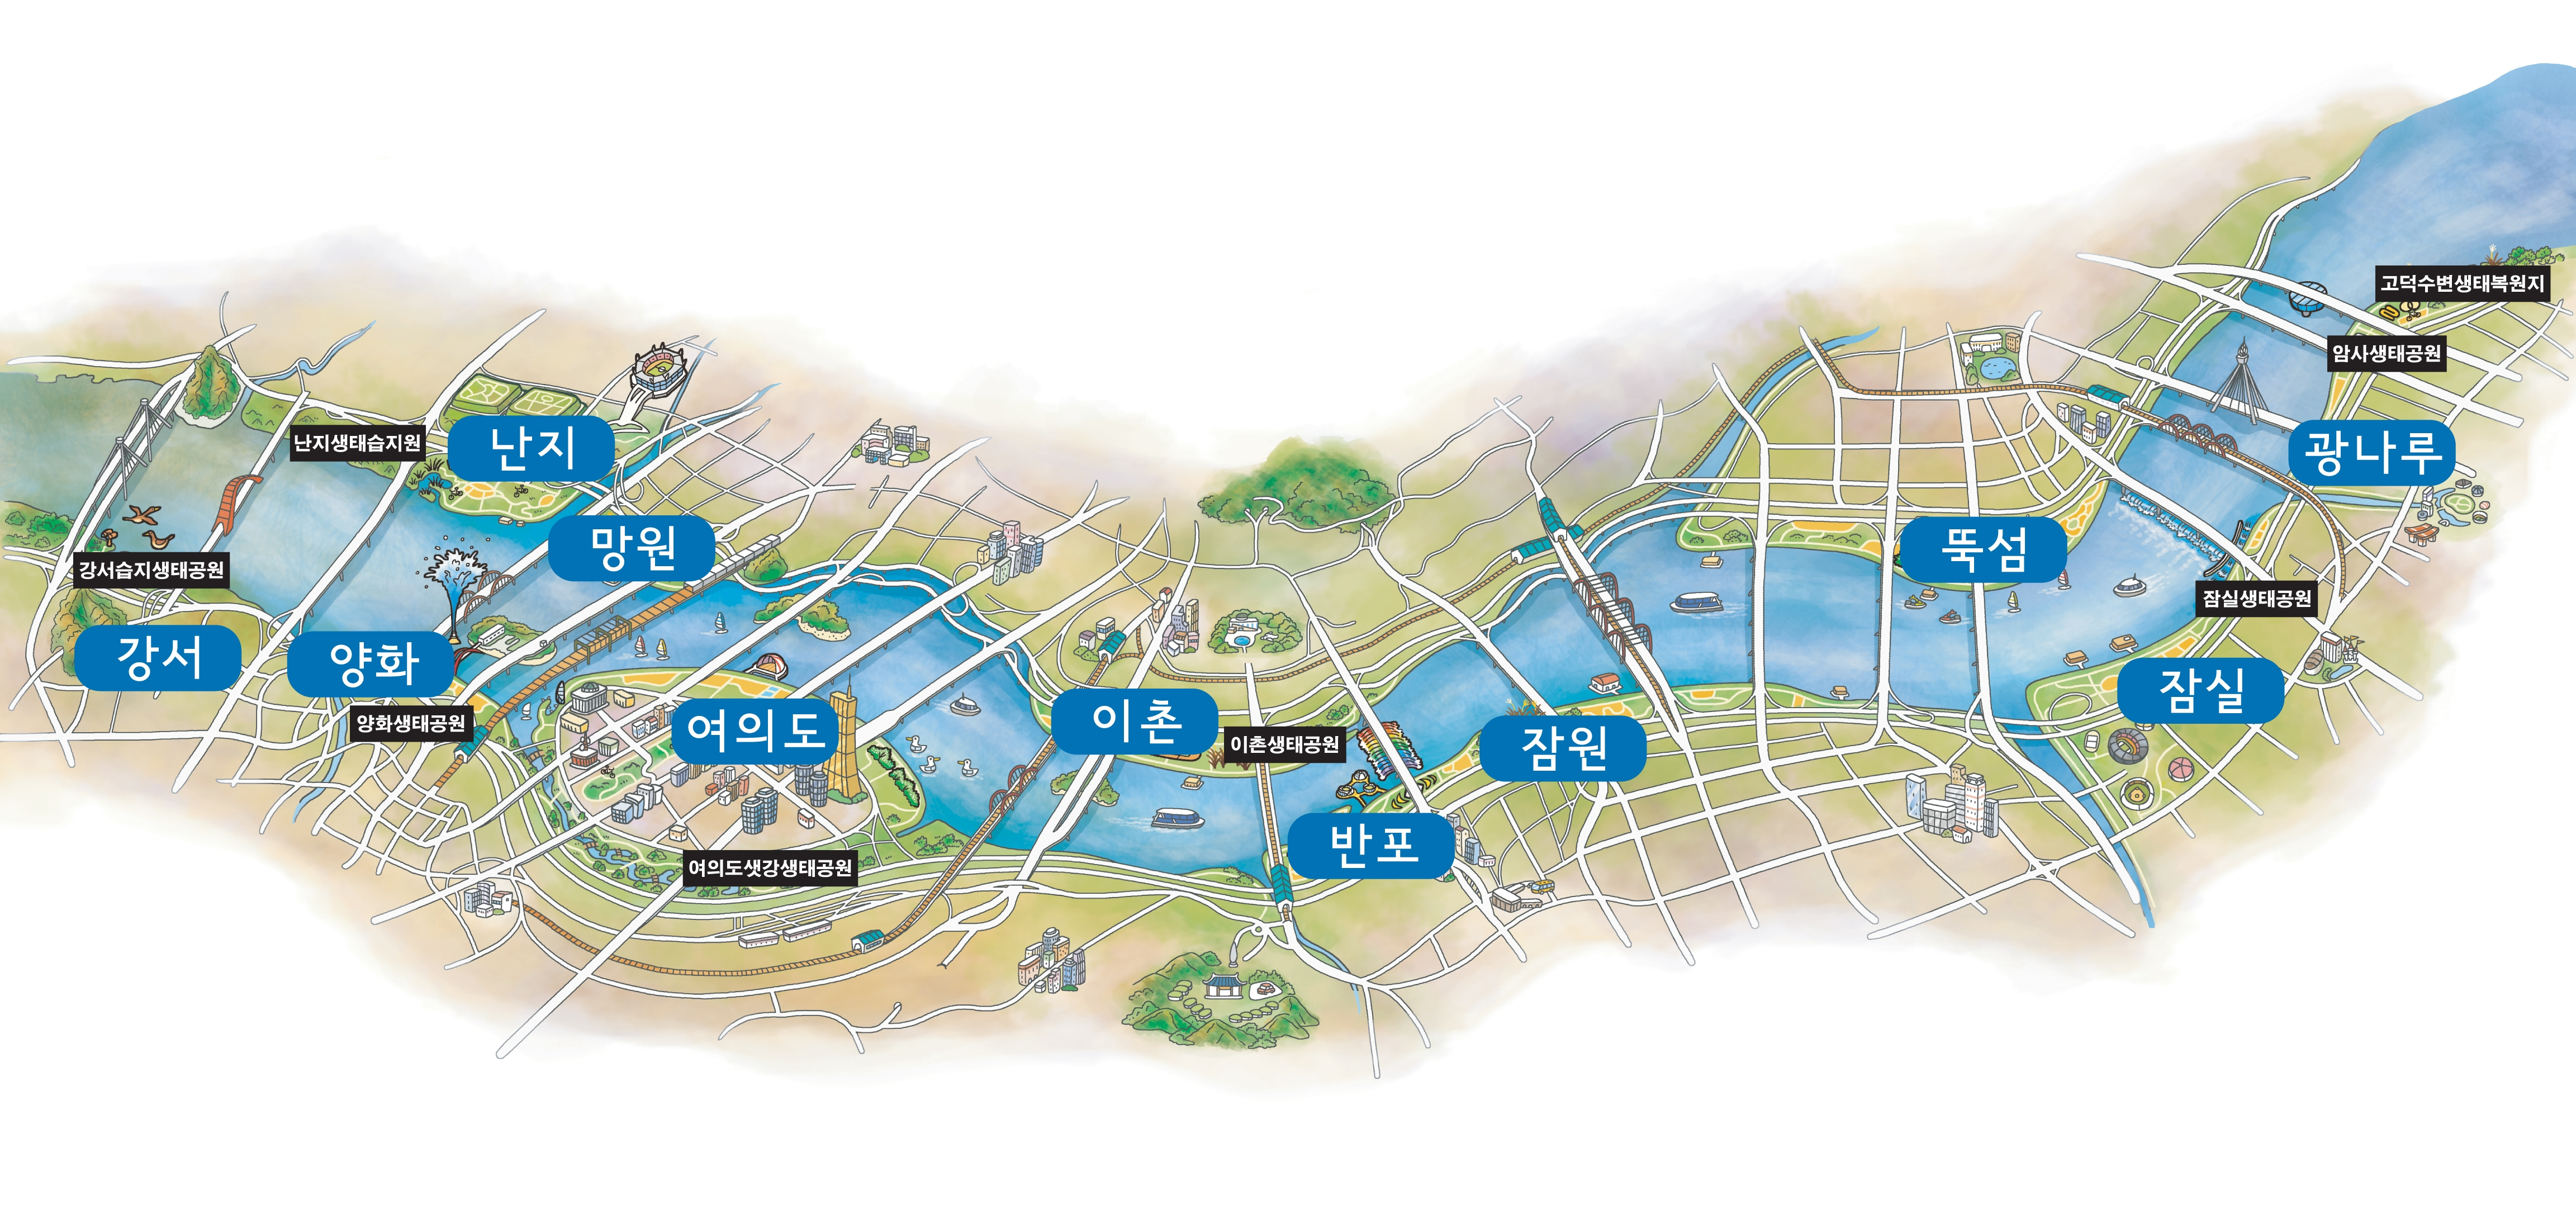
\includegraphics[width=.6\textwidth]{e_img/hanriver.jpg}
    \caption{서울의 한강공원 목록\protect\footnotemark}
    \label{fig:haryu2}
\end{figure}
\footnotetext{\href{https://hangang.seoul.go.kr/archives/9995}{서울시 한강사업본부 $>$ 한강 즐기기 $>$ 한강공원지도, 2019}}

과거의 한강 공원 지역은 강의 수위가 높을 때 잠기는 부지라고 하여 고수부지라고 
불렀으며, 80년대와 90년대에는 고수부지라는 단어가 곧 한강공원을 일컫는 단어이기도 
하였다. 그러나 고수위라는 표현은 일상적으로 잘 쓰이지 않는 용어이고, 부지가 일본식 한자
라는 비판을 받아 한강 둔치라고 고쳐 부르게 되었다. 둔치란 물가에 있는 언덕이라는 
뜻의 단어라서 강가뿐 아니라 바닷가, 호숫가에도 쓸 수 있기 때문에, 보다 정확한 표현으로
한강턱이라고 불러야 한다는 의견도 있다.



법적으로 공원녹지에 해당하며, 서울특별시 한강공원 보전 및 이용에 관한 기본조례,
서울특별시 한강공원 보전 및 이용에 관한 기본조례 시행규칙, 구리시 한강시민공원 이용시설의
설치 및 운영에 관한 조례, 구리시 한강시민공원 이용시설의 설치 및 운영에 관한
조례 시행규칙 등의 보호를 받고 있다.
\footnote{\href{https://ko.wikipedia.org/wiki/한강공원}{한강공원 $|$ 한국어 위키피디아. 2021.06.03 확인}}


\subsection{편의시설 정보}
각종 체육시설과 휴게시설이 있으며, 한강 유람선을 탈수 있는 선착장 등이 있다. 자전거
길이 잘 되어 있기 때문에 서울에서 자전거를 즐겨타는 사람들이 자전거 산책 목적으로
즐겨찾는 공간이기도 하다. 중간에 편의점들이 있는데, 봉지라면을 즉석으로 끓여주는
기기가 갖추어져 있어 이렇게 먹는 라면이 한강 라면으로 유명해지기도 했다. 봉지 라면을
뜯은 뒤, 은박지 그릇 위에 면과 스프를 넣고 물을 넣고 끓여서 먹는 방식이다. 맥주 집도 
들어서서 자전거를 옆에 두고 치맥을 즐길 수 있다.

\begin{figure}[ht]
    \centering
    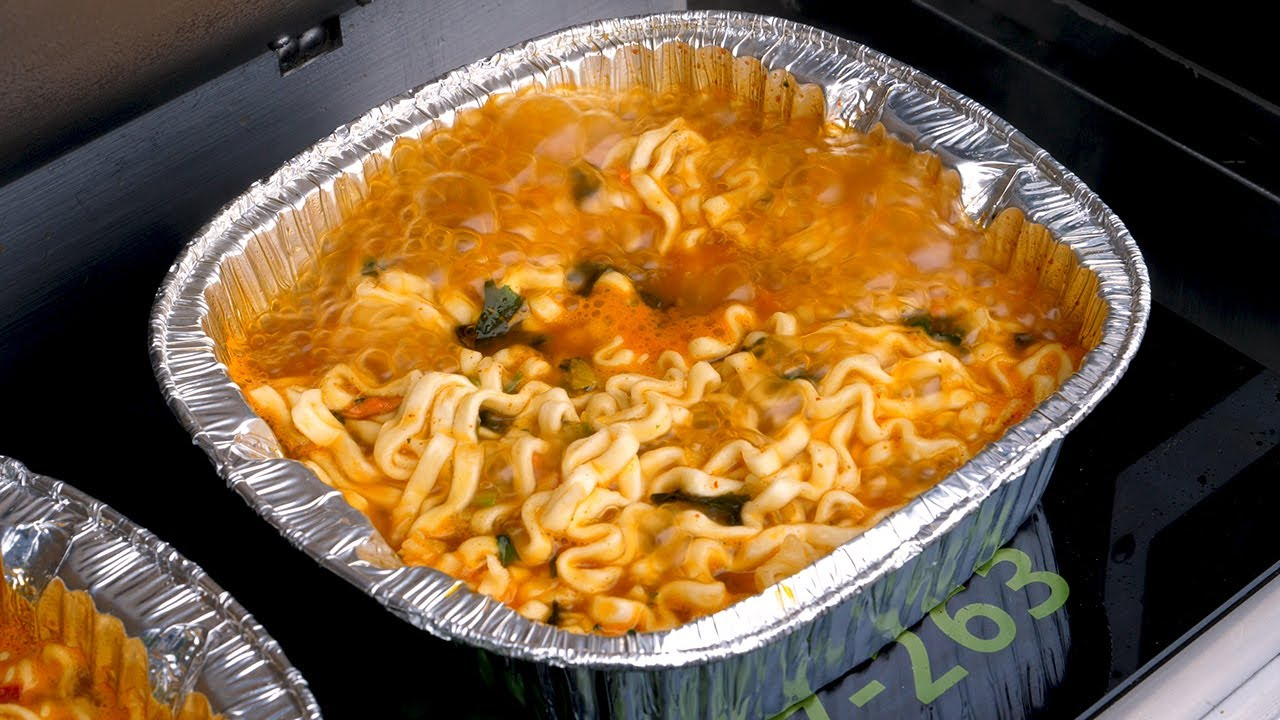
\includegraphics[width=.6\textwidth]{e_img/ww_-003.jpg}
    \caption{한강공원에서 판매하는 라면}
    \label{fig:haryu4}
\end{figure}

주말 오후에 한강 공원을 방문하면 산책로를 따라걸으며 데이트하는 커플들과 자전거를
타고 운동하는 사람들을 많이 볼 수 있다. 단 이 곳 자전거로는 시속 25km 이상의
전기 자전거나 전동킥보드는 허용하지 않으니 알아두어야 한다.

한강 둔치에 위치한 공원은 한강 공원 말고도 많지만 서울특별시에서 한강종합개발계획으로
조성한 공원만 한강 공원이라고 부른다. 때문에 경기도 한강 둔치에 위치한 구리
한강시민공원이나 남양주 한강시민공원 등은 한강공원에 속하지 않는다.


\section{한성백제 역사 유적}
송파구에 위치한 풍납토성과 몽촌토성은 서울에서도 보기 드문 훌륭한 산책 코스 중
하나인데, 이 길은 한국의 고대사에서 아주 중요한 문화유적지이고 백제의 중심지기도 했다.
고즈넉한 산책로를 걸으며 2천 년 전 백제가 꿈꾸던 서울을 알아보자.
이 탐방로의 대부분이자 가장 핵심구간이라고 할 수 있는 곳은 천호역에서 나오면 바로
만나는 풍납토성과 올림픽공원으로도 잘 알려진 몽촌토성이다. 두 개의 토성은 한국의
고대국가로 번성했던 백제의 왕성인 것이다.


백제는 지금부터 약 2000년 전 서울의 한강을 중심으로 건국해 660년에 멸망하기까지
약 700년의 역사를 가진 나라이다. 백제는 고구려, 신라와 함께 한반도에 삼국시대를
이루었으며, 가장 화려한 문화를 꽃피운 나라로 볼 수 있다. 한때 백제가 차지한 한강 유역은
일찍부터 철기문화와 농경문화가 발전해서, 백제는 다른 나라에 비해 상대적으로 풍요롭게
살 수 있었고, 이를 바탕으로 화려한 문화 예술이 발전하였다. 또 서해바다로 이어진
한강을 끼고 있던 백제는 조선기술을 발전시켜 동북아시아 해상교역의 중심국가로 부상할
수 있었다.


백제가 고구려에 패해 수도를 부여로 옮기기 전까지, 서울 송파 지역은 백제의 수도
로서 핵심 요지의 역할을 수행했다. 백제는 4세기 경 근초고왕 때에 이르러 가장 넓은 영토와 
외교적 역량을 가진 강력한 나라가 되었는데, 그 영향력이 한반도의 북쪽으로는 평양에
서 남쪽으로는 가야에 이르렀고, 일본의 규슈 지역, 중국의 요서, 산둥 지역까지 그 영향력
을 뻗쳤다고 알려져 있다 .풍납토성은 바로 이 한성백제의 초기 왕성으로 알려져 있으며,
몽촌토성은 이후에 군사 방어적 목적으로 추가로 건축된 왕성으로 밝혀져 있다. 사실 이러한
역사적 사실이 제대로 밝혀지고 알려진 것은 얼마 되지 않았다. 1997년 풍납토성에서
대규모의 유물이 출토되기 전까지 풍납토성과 몽촌토성은 백제의 성이기는 하지만 그리 
중요한 성일 것이라고 아무도 생각하지 않았다. 그러나 풍납토성에서 대규모의 백제의 
왕궁유물이 출토되면서 많은 역사학자들이 궁금해 했던 백제 초기의 왕성이 1600여 년 만에
드러난 것이다. 그래서 이 탐방로의 구간은 최근까지도 활발한 발굴과 연구조사가 진행 
중이기도 하다.

\subsection{풍납토성}


풍납토성은 그 규모와 건축 기술에서 고대 이집트의 피라미드 건축 기술을 뛰어 넘는
다. 풍납토성은 판축기법과 부엽공법을 사용해 만들었는데, 이것은 일정한 간격으로 만든
나무틀에 체로 거른 고은 흙과 나뭇잎, 그리고 뻘흙을 사용해 시멘트보다 단단한 토성을 
만들어낸 방식이다. 발굴 과정에서 드러난 풍납토성의 규모도 입을 다물지 못할 수준이다. 
풍납토성은 최대 폭이 40m, 높이 15m, 배 모양의 성곽이 3.5km 길이로 이어져 있다. 이 정도
공사를 하기 위해 10톤 트럭 15만 대(150만 톤) 분량의 흙이 필요하고, 연간 200만 
명이 동원되었을 것으로 추정된다. 백제가 초기부터 강력한 왕권 국가가 아니었다면 해낼 수
없는 대규모 국책 사업이었던 것이다.
\footnote{\href{https://ko.wikipedia.org/wiki/서울_풍납동_토성}{서울 풍납동 토성 $|$ 한국어 위키피디아. 2021.06.03 확인}}

\begin{figure}[ht]
    \centering
    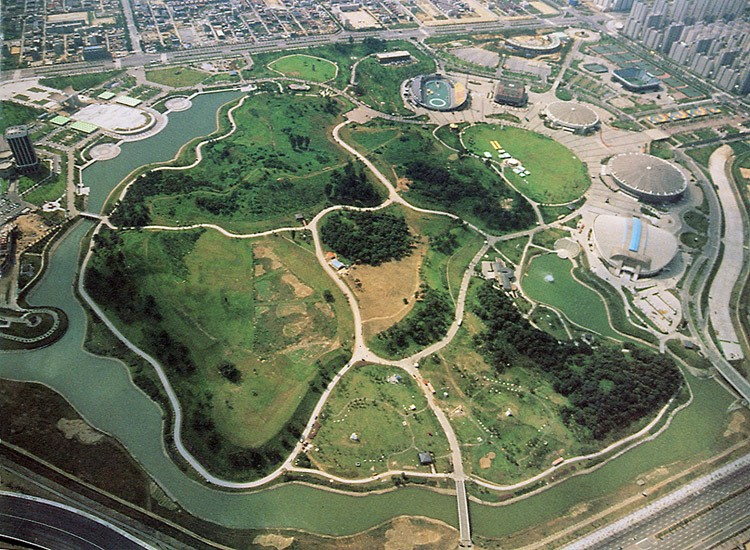
\includegraphics[width=.45\textwidth]{e_img/ww_-004.jpg}
    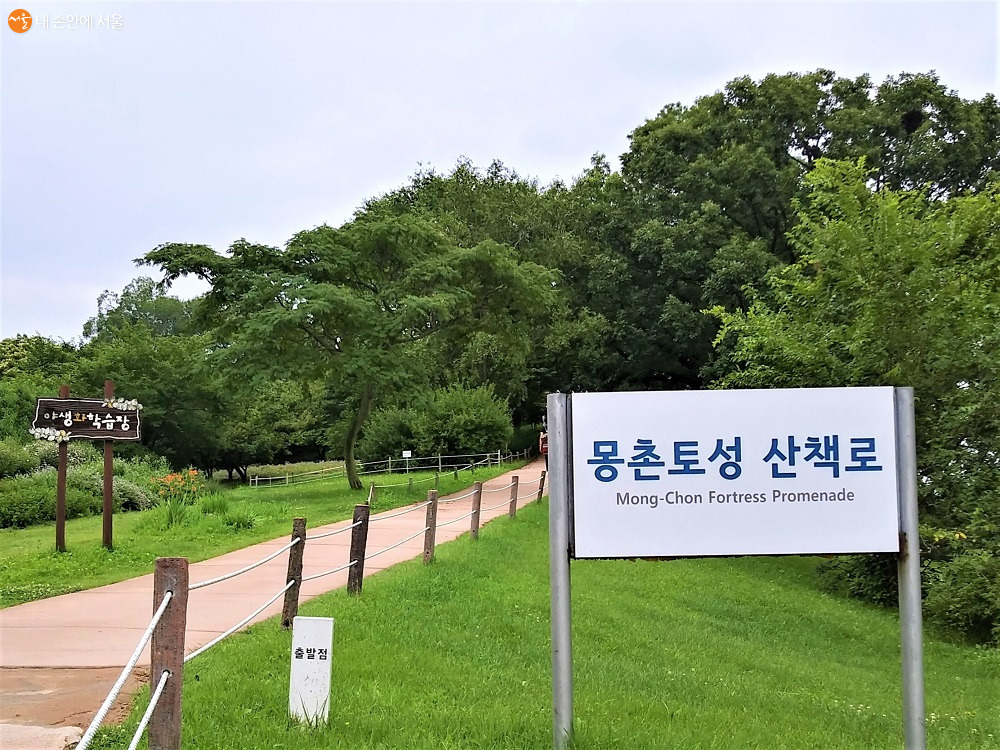
\includegraphics[width=.45\textwidth]{e_img/ww_-005.jpg}
    \caption{풍납토성(좌)와 몽촌토성(우)}
    \label{fig:haryu6}
\end{figure}

\subsection{몽촌토성}
몽촌토성은 근초고왕 시기인 4세기 전후에 축조된 백제의 왕성으로, 남한산성의 
산줄기와 한강의 자연지형을 그대로 이용해 건축되었다. 몽촌토성의 호수 역시 자연지형을
이용해 만든 해자의 흔적이다. 비록 지금은 지형이 많이 바뀌었지만, 옛 지도를 보면 
몽촌토성의 호수는 현재의 석촌 호수까지 이어져 한강의 지류를 이루고 있었다. 몽촌토성을 
만든 이유에 대해서는, 위례성의 인구가 증가하자 위례성 밖에 살고 있는 백성들을 위해 
축조했다는 의견과 함께, 초기 왕성인 풍납토성이 적의 공격에 취약해 방어성으로서 몽촌토성
을 새로 건축했다는 의견도 힘을 얻고 있다. 어찌되었든 풍납토성과 함께 몽촌토성은 
백제가 강력한 고대 국가의 기틀을 다질 수 있게 해준 왕성으로 평가받고 있다.
\footnote {\href{https://ko.wikipedia.org/wiki/서울_몽촌토성}{서울 몽촌토성 $|$ 한국어 위키피디아, 2021.06.03 확인}}



\section{선유도 공원}
방탄소년단 멤버 RM 의 `seoul'이라는 곡을 들어보면 가사에 선유도가 등장한다. 서울
사람에게 선유도 공원은 꽤 중요한 장소임이 틀림없다. 양화대교와 맞닿아 있으며, 
행정구역 상으로 영등포구 당산동과 양화동에 속해 있다.

한강 중심부에 자리한 작은 봉우리섬 선유도는 예로부터 빼어난 풍광을 지닌 곳으로
예술가와 묵객시인들의 사랑을 받은 곳이었다. 그러나 일제강점기를 거치며 선유봉의 옛
모습은 사라졌고, 1978년부터 2000년까지 서울 서남부 지역에 수돗물을 공급하는 
정수장으로 사용되었다. 이후 2002년 4월 다양한 볼거리와 즐거움을 선사하는 
친환경생태공원으로 재생되었다.


\begin{figure}[ht]
    \centering
    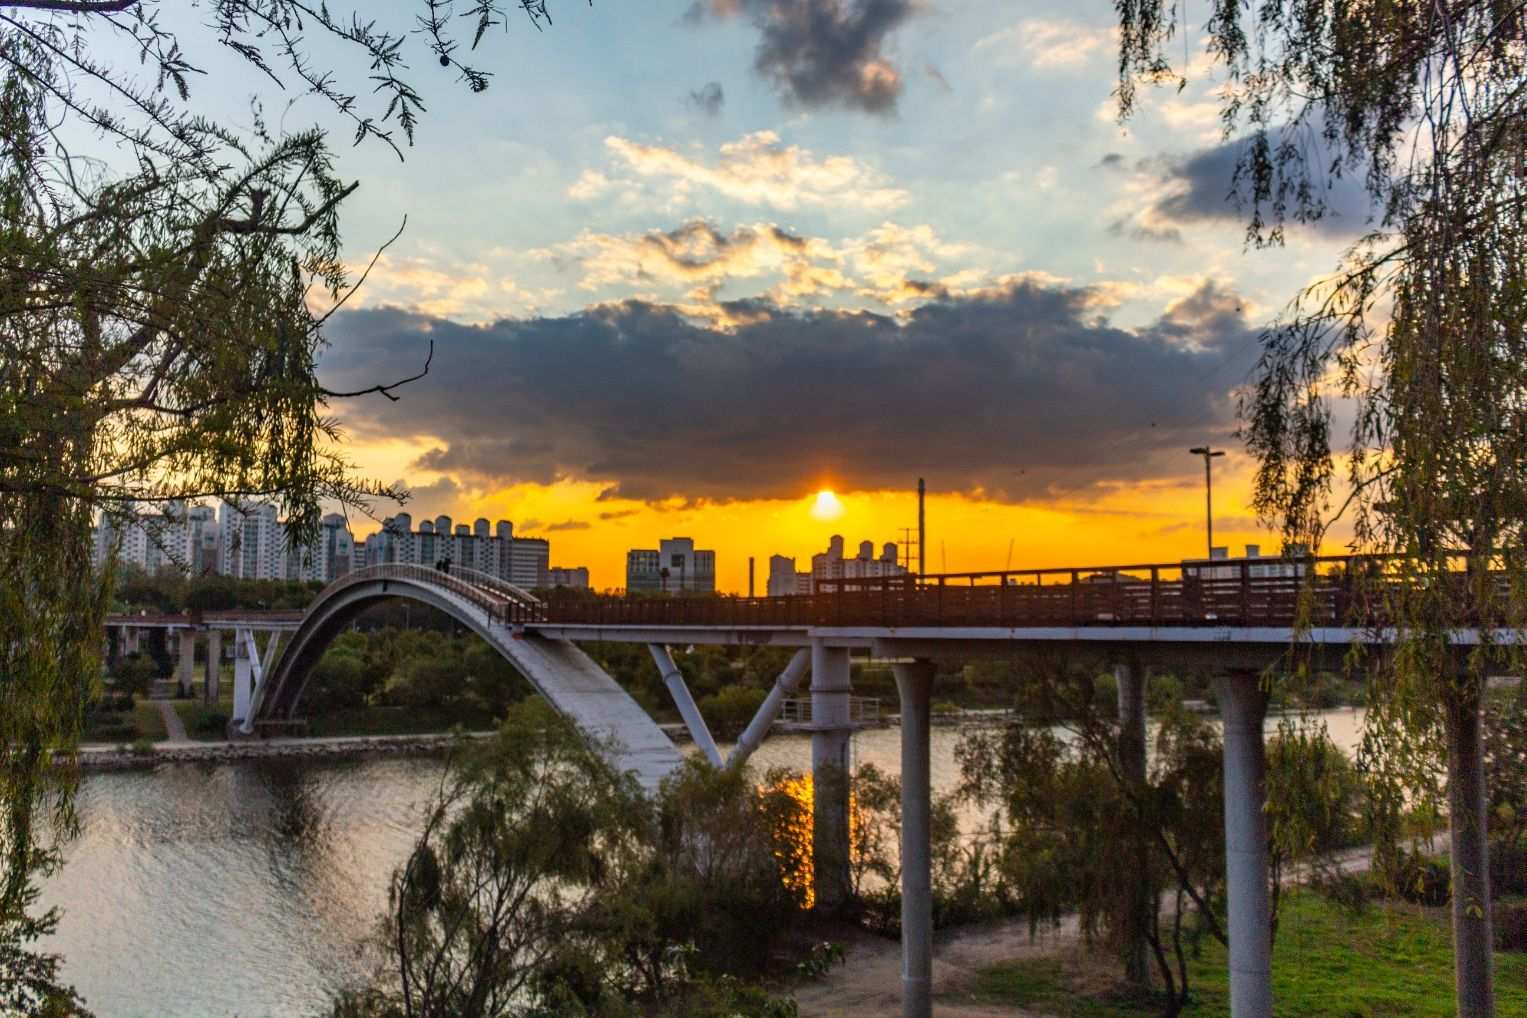
\includegraphics[width=.6\textwidth]{e_img/ww_-006.jpg}
    \caption{선유도 공원의 일몰}
    \label{fig:haryu7}
\end{figure}

카페와 식당이 안에 있다. CU 편의점 선유도점이 열었다가 문을 닫았고, 지금은 
나루라는 카페테리아가 영업 중이다. 커피 맛에 민감한 사람이라면 추천하지 않는다. 한강 
건너편에는 한강시민공원 양화지구가 있다. 무지개다리라 불리는 선유교를 통해 직접 건널 수
있으며, 야간이 되면 무지개빛 형광을 띠는 볼거리를 선사한다. 비탈길을 갖추어 놓았지만
그것은 노약자와 정비차량을 위해 마련된 것으로, 자전거로는 통행할 수 없다.


이 외 한강전시관, 수질정화원, 환경물놀이터, 녹색 기둥이 있는 정원, 수생식물원,
시간의 정원,원형소극장 등의 공간을 볼 수 있다. 선유도는 느즈막한 노을 시간대와 밤 
시간대의 야경이 특히 아름답다.
\footnote{\href{https://ko.wikipedia.org/wiki/선유도공원}{선유도공원 $|$ 한국어 위키피디아. 2021.06.03 확인}}


\section{저녁: 서울신라호텔 팔선 중식당}


\begin{figure}[ht]
    \centering
    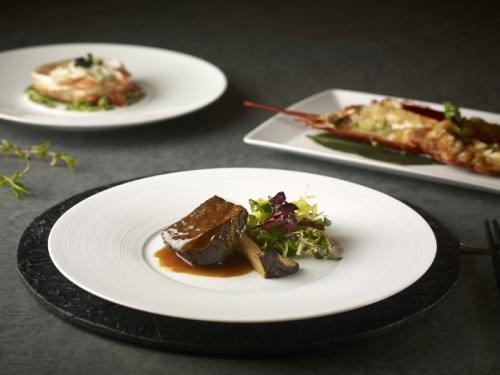
\includegraphics[width=.6\textwidth]{e_img/ww_-007.jpg}
    \caption{팔선 중식당의 코스요리}
    \label{fig:haryu8}
\end{figure}


우리나라 부자들은 대부분 부동산 투자로 부를 축적하였다. 비트코인과 주식이 단기
투자를 통해 엄청난 이득을 낼 수 있는 것 같아도, 주요 도시에 위치한 부동산만큼의 안정
적인 상승세를 보장하지 못한다. 한국의 역사를 관통하고 있는 한강 근처는 서울시에서 
가장 집 값이 높은 지역이며, 교통과 편의 그리고 배산임수가 잘 고려된 대한민국 최고의 
거주지라는 평가를 받는다.

서울을 떠나기 전 고급스럽기로 손에 꼽히는 서울신라호텔 팔선 중식당에서 식사해
보는 것을 추천한다. 중식이지만 한국의 문화가 잘 반영되어 있으며, 영어 등 외국인을 위
한 메뉴판이 준비되어 있다. 세트 메뉴는 인당 20만원 수준으로 가격대가 있는 편이지만,
3만원 이내의 면류나 10만원 이내의 메인 디쉬를 고를 수 있고 이 외에도 선택지가 다양하다.



\section{강화해협}


인천 강화군 강화도는 답사의 일번지, 우리 역사의 전시장 등으로 불리는데, 유적과
유물이 많고, 중요한 역사적 사건이 많이 발생했다. 국내, 국제 무역을 위한 해선들이 
서울로 진입하기 위해 반드시 거쳐야 하는 첫 번째 관문이었다.

\begin{figure}[ht]
    \centering
    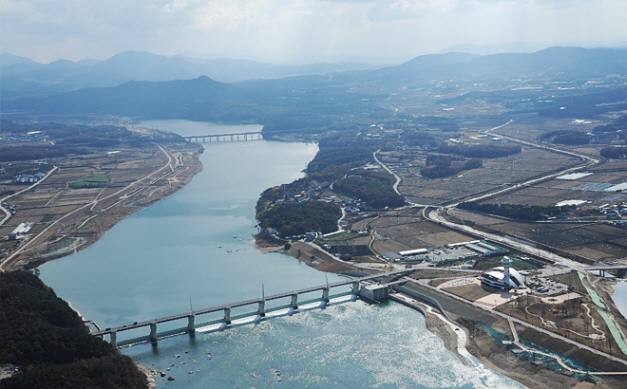
\includegraphics[width=.6\textwidth]{e_img/ww_-008.jpg}
    \caption{강화해협의 모습}
    \label{fig:haryu9}
\end{figure}


한강에 관심 있는 사람이라면 염하라는 말을 들어본 적이 있을 것이다. 염하는 강화
해협을 이르는 말로, 프랑스 병인양요 시기 프랑스의 1차 보복 전 원정 과정 중, 프랑스 신
부와 갑구지 촌로 사이의 잘못된 통역으로 인해 짠 물로 해석되어 지금까지 전해져 내려오
고 있다고 알려져 있다. 서해안의 조수간만의 차가 큰 까닭에 배를 타고 이 곳을 지나기는
쉽지 않으며, 밀물과 썰물 때는 물살이 아주 세차게 흐르는 곳이기도 하다. 해협을 가로질
러 강화대교와 강화초지대교가 해협 위에 건설되어 있다. 과거에는 배를 타고 한강으로 들
어가는 통로였기에 아주 중요한 해상교통로의 역할을 했다. 그 흔적으로 강화해협 주변에
진, 보, 돈대, 포대 등 많은 군사시설들이 산재해 있음을 볼 수 있다.

